
% Original template by Andrew G. West - prop_spec.tex
% Document by Cris Feo and Ben Perez
% Main LaTeX file for CIS400/401 Project Proposal Specification
%

	%	% AW - Ordinarily we'd begin by specifying some broad document properties like font-size, page-size, margins, etc. -- We have done this (and much more) for you by creating a 'style file', which the 'documentclass' command references.
\documentclass{sig-alternate}
 
	% AW - These 'usepackage' commands are a way of importing additional LaTeX styles and formattings that aren't part of the 'standard library'
\usepackage{mdwlist}
\usepackage{url}

\begin{document} 

	% AW - We setup the parameters to our title header before 'making' it.
\title{Semi-Supervised Wikipedia Category Suggestion}
\subtitle{}
\numberofauthors{4}
\author{
	\alignauthor Benjamin Perez \\ \email{bperez@seas.upenn.edu} \\ Univ. of Pennsylvania \\ Philadelphia, PA
	\alignauthor Cristoforo Feo \\ \email{cfeo@seas.upenn.edu}   \\ Univ. of Pennsylvania \\ Philadelphia, PA
\and
	\alignauthor Andrew G. West \\ \email{westand@cis.upenn.edu} \\ Univ. of Pennsylvania \\ Philadelphia, PA
	\alignauthor Insup Lee      \\ \email{lee@cis.upenn.edu}     \\ Univ. of Pennsylvania \\ Philadelphia, PA
}
\date{}
\maketitle


	% AW - Next we write out our abstract -- generally a two paragraph maximum, executive summary of the motivation and contributions of the work.
\begin{abstract}
\textit{In 2005 Wikipedia implemented a category system for the purposes of facilitating navigation throughout the site. Since then, it has grown to 1.5 million categories covering over four million articles. Currently, all categorization of articles on Wikipedia is done by human editors---A task which involves an enormous amount of repetitive work.}

\textit{This paper proposes building an automated system that suggests missing category-article links to editors through a browser-based user-interface. This system will utilize the existing corpus of human-categorized articles, as well as available metadata, to provide a ranked list of suggested categorizations. All suggested categorizations are subject to final approval or rejection by a human editor.}
\end{abstract}


	% AW - Then we proceed into the body of the report itself. The effect of the 'section' command is obvious, but also notice 'label'. Its good practice to label every (sub)-section, graph, equation etc. -- this gives us a way to dynamically reference it later in the text via the 'ref' command.
\section{Introduction}
\label{sec:intro}
Fundamentally, Wikipedia consist of a number of content pages, or articles, and a series of categories to which articles might be linked. Categories may have sub categories and pages may belong to several different categories. In a traditional knowledge base this format works well for classifying all manner of different objects. If a new object is to be added, the editors will follow whatever criteria they have laid out for placing items into their correct categories. However, the unique nature of Wikipedia as a massively collaborative resource presents an interesting challenge for categorization~\cite{Richardson}. In particular all editing is performed by volunteers who are wildly diverse in terms of geography, education, and professional interests. While this is great for the collection of knowledge in general, it is not ideal for categorization---where there are many opportunities for misunderstanding~\cite{McDonald}.

Take, for example, the Wikipedia page for "George Washington". Suppose an editor writes this article and categorizes it under "Presidents of the United States". Later, another author comes along and writes an article on "James Monroe", deciding to create a new category for "People from Westmoreland County, Virginia". Now unless someone visits the "George Washington" article and previously knows that the "Westmoreland County" category exists they will think nothing of it and that missing category link will go unnoticed. These kinds of missing links exist in many places on Wikipedia and are incredibly difficult to detect through casual browsing. The category system itself suffers from a number of ambiguities that make this a difficult problem to solve. Perhaps the greatest is a fundamental disagreement over how categorizations should work first identified by Thornton~\cite{Thornton}. She noted that the two ways of looking at categories, hierarchical and relational, are both currently used by Wikipedia. This makes automated category suggestion relatively difficult with traditional machine learning techniques that attempt to extract a single type of semantic meaning from article categorizations.

In spite of this, it is clear that the category system serves its purpose as a navigational tool tying together articles that share some measure of similarity. Therefore, we plan to utilize an approach that leverages the existing pseudo-hierarchical category structure of Wikipedia as a guide. In fact this is exactly what the recommended procedure for categorizing new articles suggests: "One way to determine if suitable categories already exist for a particular page is to check the categories of pages concerning similar or related topics."~\cite{cattalk} It is our goal to create a tool which will find these missing category links and bring them to the attention of editors so that they might be quickly and easily added. This will benefit the category system as a whole and potentially simplify the categorization process for a wider audience of editors~\cite{Fu}.
\begin{figure*}[htb!]
	\begin{center}
		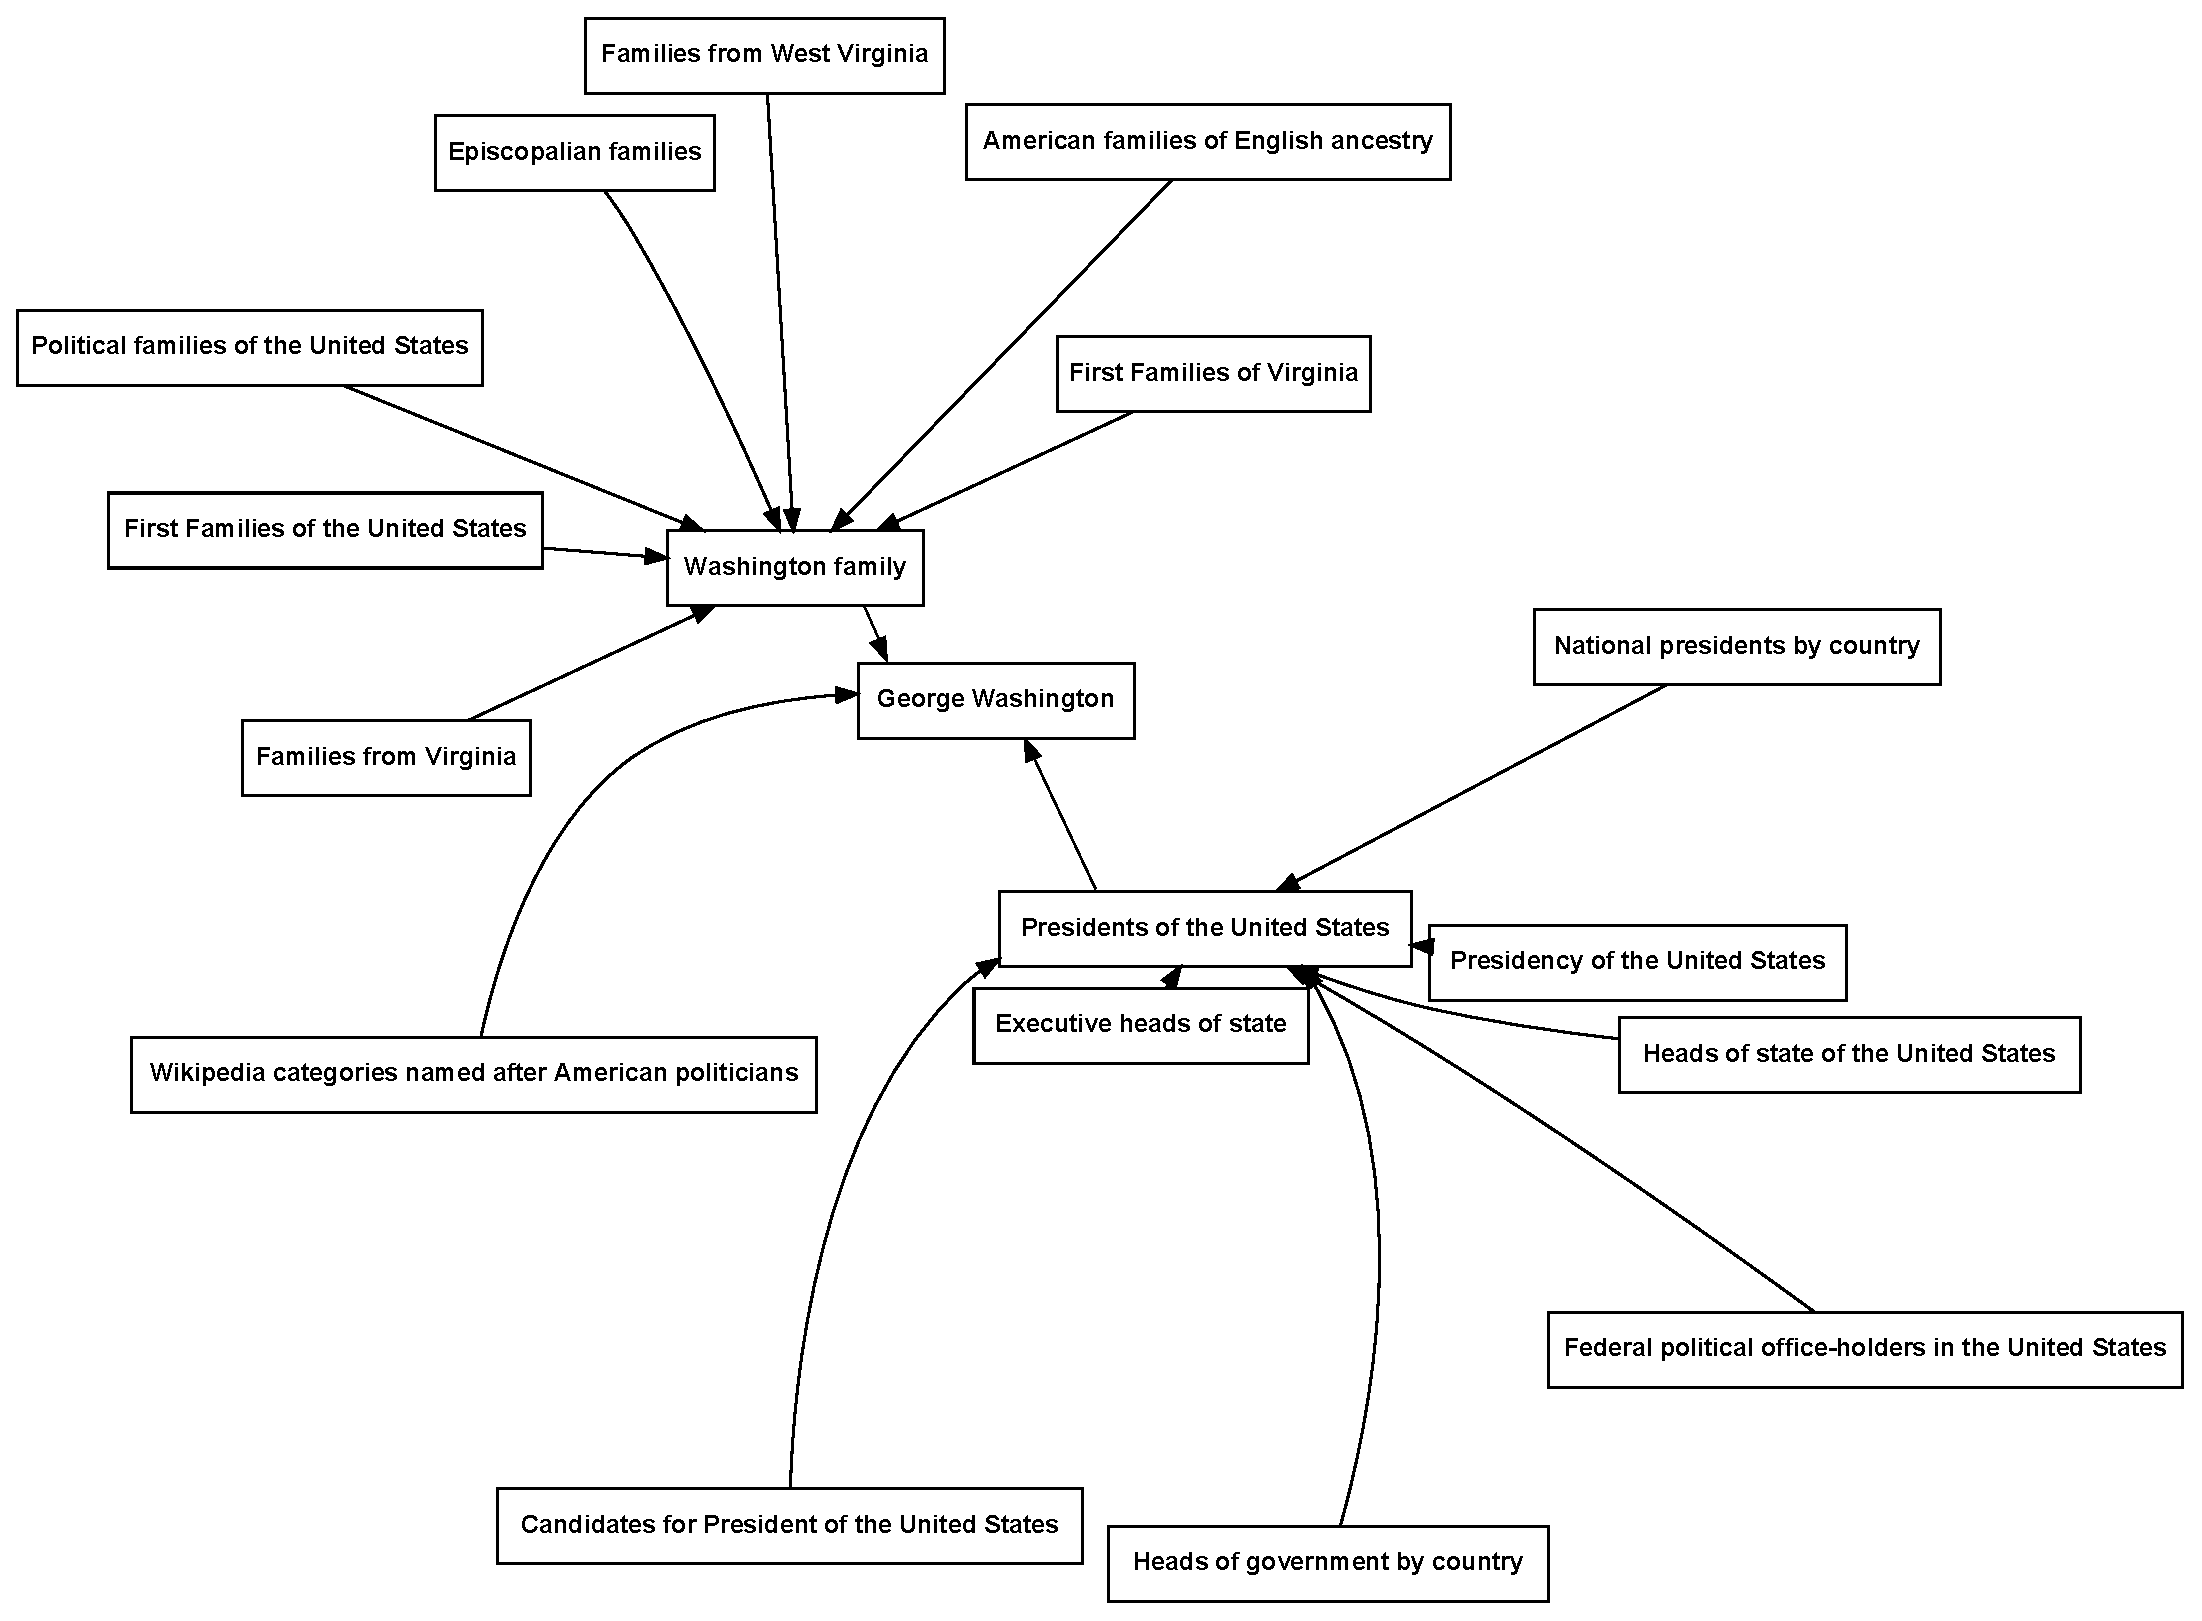
\includegraphics[width=1.0\linewidth]{washington-graph}
	\end{center}
	\vspace{-12pt}
	\caption{A small part of the category heirarchy for the Wikipedia article on "George Washington".}
	\label{fig:washington-graph}
\end{figure*}


	% AW - The header of this document might have been a little intimidatating to beginners. Notice once you are in the body of the document, however, LaTeX commands are minimal and 'normal text' is frequent.
\section{Related Work}
\label{sec:related_work}
Because Wikipedia is such a rich, diverse corpus of information, a lot of areas of machine learning research use Wikipedia as a training set for a variety of learned models. In this way, Wikipedia is used to improve the quality of machine learning research. We are proposing to do the opposite: to use machine learning techniques to improve the quality of Wikipedia.

Automated classification of Wikipedia categories is an area that has been studied from several different angles. The category system contains a huge amount of extractable information, although it is very loosely structured~\cite{Ponzetto,Strube}. The most simplistic approaches to categorizing Wikipedia utilize supervised learning. Supervised learning takes as input a set of training examples and their associated labels. In our case, these training examples are Wikipedia articles and their labels are the categories associated with them. Supervised learning uses these labeled training examples to learn a model which can predict the labels of previously unseen examples~\cite{Szymanski}.

There are two broad groups of features which are used as input to supervised learning algorithms: content features and network features. Content features reflect information directly contained within a given page. Examples of content features include textual keywords, infobox information, and metadata associated with a specific article~\cite{Tkachenko}. Network features describe the hyperlinked graph of Wikipedia articles and may contain information such as the number of outgoing links, the number of incoming links, and properties of neighbors in this hyperlinked graph~\cite{Getoor}.

The use of content features or network features alone has yielded impressive results. Using a combination of both feature types has been shown to be even more effective~\cite{Gantner}. Although supervised learning techniques are highly accurate for a few very specific categories~\cite{Gantner, Fu, Szymanski, Tkachenko}, they suffer from problems of scale. This is primarily because a classifier must be trained for each and every category. This approach will clearly not scale across the entire category system of Wikipedia, with its large and constantly changing set of categories~\cite{Fu}. Furthermore, previous work demonstrated that supervised learning is best for distinguishing between a few very distinct categories. This assumption does not hold across the vast majority of the category system, where categories may overlap or contain subtle differences~\cite{Thornton}. All of these limitations arise because supervised learning works primarily at the level of individually labeled articles, fundamentally limiting the amount of information that can be incorporated from the entire Wikipedia graph, even when network features are included.

Another approach to categorizing Wikipedia is to use semi-supervised learning algorithms. Semi-supervised learning differs from supervised learning in that it uses unlabeled data in the learning process. Many of these methods rely on label-propagation across a graph. The input to a semi-supervised learning algorithm is generally a set of examples. This set of examples is divided into labeled and unlabeled data. Using the assumption that the data are distributed in a way which correlates with their labels, the missing labels in the data can be estimated~\cite{Carlson}.

Azran describes a generic example of an algorithm---known as the rendezvous algorithm---which can estimate a multi-class distribution of labels across examples. The rendezvous algorithm works by treating each example as a node in a fully connected graph. Each edge in this graph has an associated weight which is given by its entry in a pairwise similarity matrix between all examples called the transition matrix. Labeled example nodes are set to be absorbing states and unlabeled example nodes are set to be emitting states in a Markov random walk. After running a number of random walks for each node, the distribution of labels for that node can be inferred by looking at the distribution of absorbing states for its random walks~\cite{Azran}.

Chidlovskii describes the results of a related random walk algorithm on Wikipedia. One of the important concerns he raises is the difficulty of computing a pairwise similarity matrix for a dataset as large as Wikipedia. One way to avoid this problem is to use the graph of hyperlinks between pages as a starting point for the transition matrix. Although the specifics of Chidlovskii's algorithm differ from the rendezvous algorithm, they demonstrate that label-propagation approaches have enormous potential in sparse graph applications such as Wikipedia~\cite{Chidlovskii}.

Graph based approaches such as these avoid the scalability bottleneck of needing to train an individual classifier for each category on Wikipedia. Furthermore, they allow us to incorporate all of the information inherent in the hyperlink structure of Wikipedia in our inference~\cite{Avrachenkov}. This link structure between articles has been found to be very highly correlated with the link structure of categories~\cite{Ponzetto, Holloway}, leading us to believe that it will be quite useful.

We plan to build off of the preliminary results described here to develop a label propagation technique which can scale to the entire Wikipedia dataset. We believe that we can combine the robust, multiclass nature of a technique like the rendezvous algorithm with approaches for dealing with scalability similar to those Chidlovskii describes to produce a superior classification system.

\section{Project Proposal}
\label{sec:project_proposal}
Our approach to this problem is twofold: first pare down the input data to a more reasonable subset of potential article-category pairings. Then apply machine learning techniques using features gleaned from each pairing to create a decision tree which outputs a confidence in the correctness of the missing link. We then plan to integrate these results into a browser-based plugin which can provide a ranked list of the potential categorizations to editors as they browse through Wikipedia.

\subsection{Anticipated Approach}
\label{subsec:approach}
Our plan to formulate ranked suggestions consists of a rough, graph-based "first-pass" which will provide potential missing categorizations in a graph of articles. At the moment we are looking into the random-walk-based technique of the Rendezvous Algorithm~\cite{Azran}. In any case the final result should exhibit high recall while still significantly reducing the number of possible categorizations for an article~\cite{Avrachenkov}. These potential article-category pairings will be used later as a basis for feature selection.

Next we take a statistically sampled subset of these potential categorizations and have individuals---ideally Wikipedia editors themselves, if we can recruit them---label each article-category pair as either good or bad.
This labeled data is then split and one portion set aside for testing. The other portion is using in training the machine learning tool Weka. We determine a number of features for article-category pairs and use them along with the labellings as input to Weka. By analyzing the output we then experimentally pare down the input features to a relevant subset which provides us with good accuracy and recall. This is expected to be a time consuming part of the project not just because training Weka on a wikipedia-scale data set is slow but also because we will need to conduct a lot of testing to balance over and under training on the labelled data.

Finally if time allows and our techniques are robust enough we plan to make our data available to editors by integrating with the popular tool Hotcat---which eases category management for Wikipedians. It is our plan to offer a simple ranked list of the top five or so potential categorizations for an article such that an editor visiting a page can quickly glance at our tool and check whether any of the supplied categories are appropriate.
\begin{figure*}[htb!]
	\begin{center}
		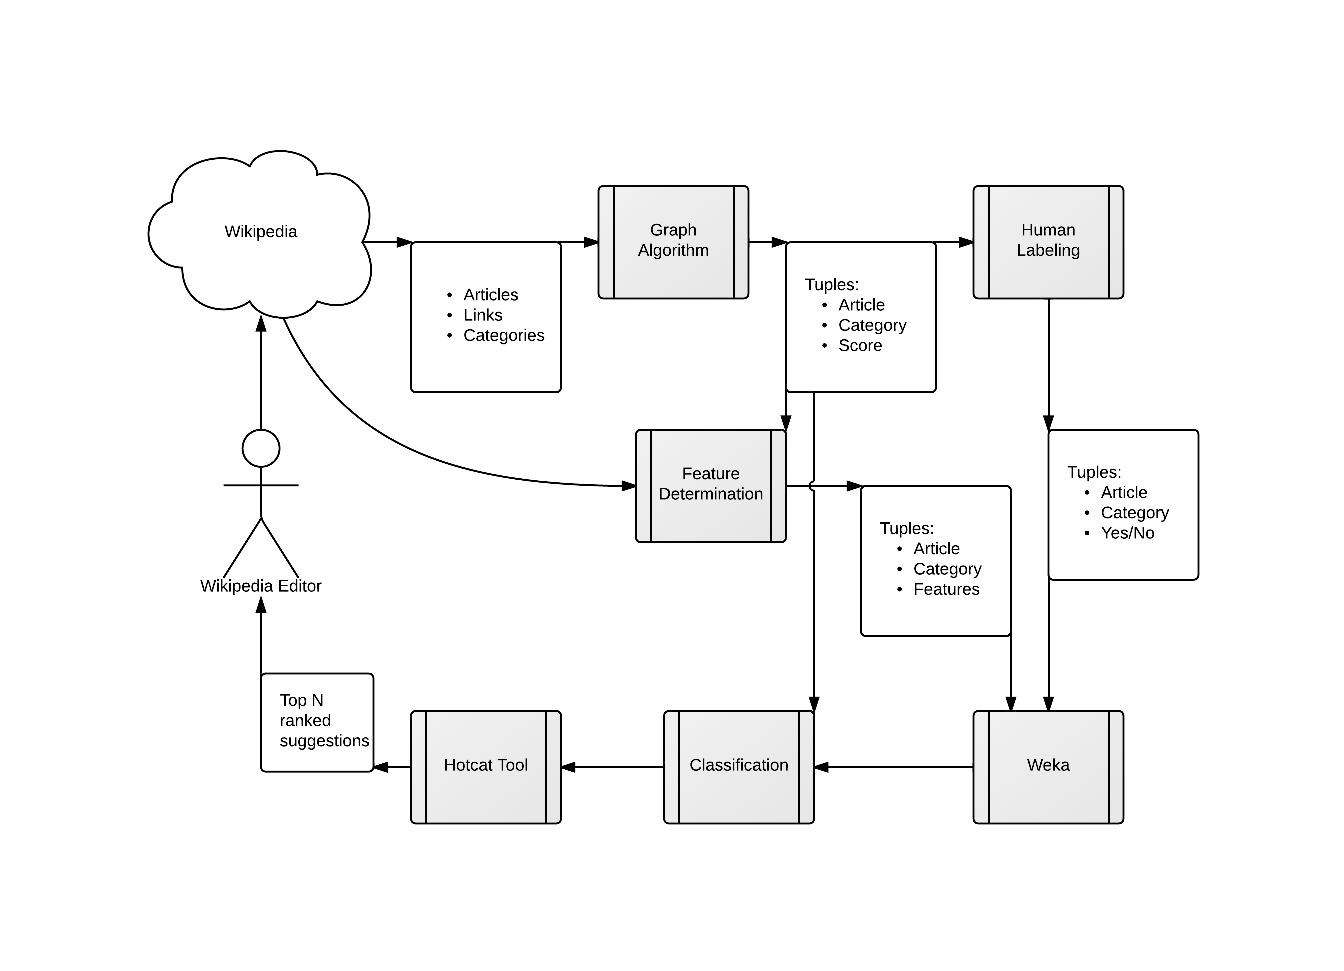
\includegraphics[width=1.0\linewidth]{block_diagram}
	\end{center}
	\vspace{-12pt}
	\caption{Our proposed system architecture. Gray blocks are processes, while arrows and white blocks represent data interchance between components.}
	\label{fig:block_diagram}
\end{figure*}

\subsection{Technical Challenges}
\label{subsec:tech_challenges}
The main technical challenges that we anticipate are related to the scale of existing Wikipedia category data. The extremely large number of categories and pages will make efficiently representing the graph in terms of memory a possible challenge. Another issue that arises from the large scale of Wikipidia data is the need for algorithms that are efficient in terms of runtime. 

\subsection{Evaluation Criteria}
\label{subsec:eval_criteria}
Evaluation of our results may be broken down into two cases: How do you know when the tool is suggesting a bad categorization and how do you know when it is suggesting a good categorization? To check that our technique is not suggesting bad links, we take the unseen portion of the labeled data which we set aside earlier and test against that. Along with testing on the labeled data, we can check that the tool is suggesting good categorizations by running the graph based-approach over an unlabeled sample with several categorizations removed and check that our algorithm recommends these missing edges with a high probability. Both of these metrics will be part of the experimental "feature-determination" portion of our project. Finally, if we tie our system into a browser then there is the potential to collect user feedback on how our tool perfroms "in the wild", although that is further down the road. A similar approach to evaluation is taken by Sunercan et al.  to evaluate the effectiveness of suggested hyperlinks between pages~\cite{Sunercan}.

\section{Research Timeline}
\label{sec:research_timeline}
\begin{itemize*}
	\item {\sc Already Completed}: We have gathered an extensive amount of related research and conducted preliminary research into potentially applicable graph algorithms. We have also set up a mySQL database and imported Wikipedia category, link, and article data.\vspace{3pt}
	\item {\sc By Thanksgiving}: We want to have a good enough understanding of our approach to the graph-based first pass so that we can decide on how to represent the graph in an efficient way and begin that implementation.\vspace{3pt}
	\item {\sc By Christmas}: Have the graph-based portion of the project up and running and begin looking into methods of tagging the output data, whether that be via actual Wikipedia editors, Mechanical Turk, etc.\vspace{3pt}
	\item {\sc By Early February}: We want to have obtained the tags for the article-category pairs by whatever means we decide on. During this time we can create the list of potential input features and set up the testing environment for Weka.\vspace{3pt}
	\item {\sc By Late March}: Have determined a minimal set of useful features and continue testing. Begin organizing ideas for final writeups and work on integration with Hotcat if there is time.\vspace{3pt}
	\item {\sc Final Tasks}: Finish the project writeup and Complete integration with Hotcat. Try to get Wikipedia editors to try the tool out. Collect feedback from editors and incorporate it into conclusion of writeup.
\end{itemize*}

	% AW: We next move onto the bibliography.
\bibliographystyle{plain} % Please do not change the bib-style
\bibliography{proposal}  % Just the *.BIB filename
\nocite{*}

\end{document} 

